\documentclass{article}
\usepackage{tikz}

\begin{document}

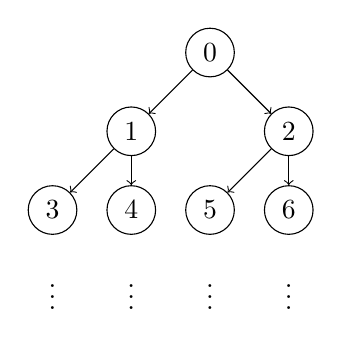
\begin{tikzpicture}[node distance=1cm]
    % Nodes
    \node[circle,draw] (0) at (0,0) {$0$};
    \node[circle,draw] (1) at (-1,-1) {$1$};
    \node[circle,draw] (2) at (1,-1) {$2$};
    \node[circle,draw] (3) at (-2,-2) {$3$};
    \node[circle,draw] (4) at (-1,-2) {$4$};
    \node[circle,draw] (5) at (0,-2) {$5$};
    \node[circle,draw] (6) at (1,-2) {$6$};

    % Edges
    \draw[->] (0) -- (1);
    \draw[->] (0) -- (2);
    \draw[->] (1) -- (3);
    \draw[->] (1) -- (4);
    \draw[->] (2) -- (5);
    \draw[->] (2) -- (6);

    % Vertices labels below
    \node[below of=3] {$\vdots$};
    \node[below of=4] {$\vdots$};
    \node[below of=5] {$\vdots$};
    \node[below of=6] {$\vdots$};

    \end{tikzpicture}

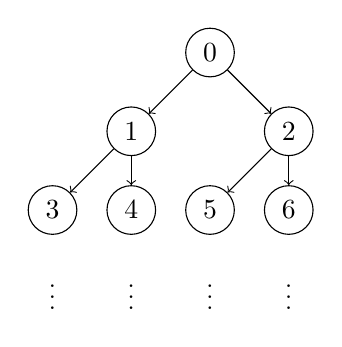
\begin{tikzpicture}[node distance=1cm]
    % Nodes
    \node[circle,draw] (0) at (0,0) {$0$};
    \node[circle,draw] (1) at (-1,-1) {$1$};
    \node[circle,draw] (2) at (1,-1) {$2$};
    \node[circle,draw] (3) at (-2,-2) {$3$};
    \node[circle,draw] (4) at (-1,-2) {$4$};
    \node[circle,draw] (5) at (0,-2) {$5$};
    \node[circle,draw] (6) at (1,-2) {$6$};

    % Edges
    \draw[->] (0) -- (1);
    \draw[->] (0) -- (2);
    \draw[->] (1) -- (3);
    \draw[->] (1) -- (4);
    \draw[->] (2) -- (5);
    \draw[->] (2) -- (6);

    % Vertices labels below
    \node[below of=3] {\small $\vdots$};
    \node[below of=4] {\small $\vdots$};
    \node[below of=5] {\small $\vdots$};
    \node[below of=6] {\small $\vdots$};

\end{tikzpicture}

Each vertex $j$ for $2^k-1\le j\le 2^{k+1}-2$ may be reached in exactly $k$ steps.
\end{document}